\section{Multi-Layer Perceptron}
\begin{frame}[c]{Multi-Layer Perceptron}
    \begin{figure}
        \captionsetup[subfigure]{labelformat=empty, font={color=black}}
        \begin{subfigure}{0.6\textwidth}
            % trim=left bottom right top, clip
            \centering
            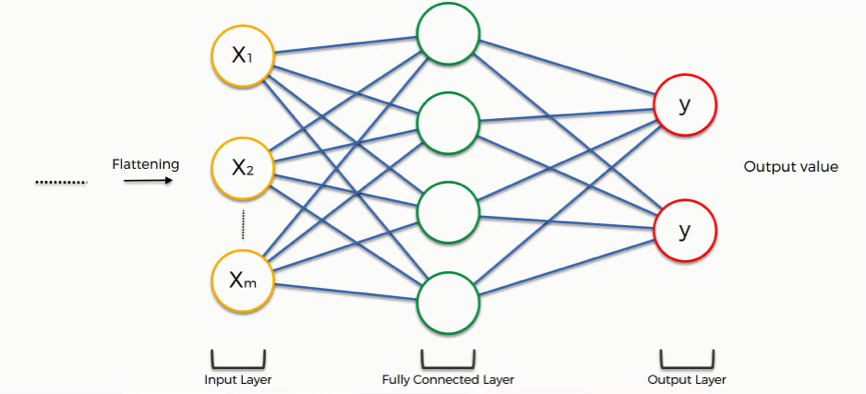
\includegraphics[width=0.7\textwidth,trim=90 0 60 0,clip]{dense_layer}
            \caption{Multi-Layer Perceptron with one fully connected layer. Alternative names include 'dense', 'fully connected' and 'mlp' layer. Figure from \cite{BibEntry2018Aug}.}
        \end{subfigure}
        \hspace{3em}
        \begin{subfigure}{0.3\textwidth}
            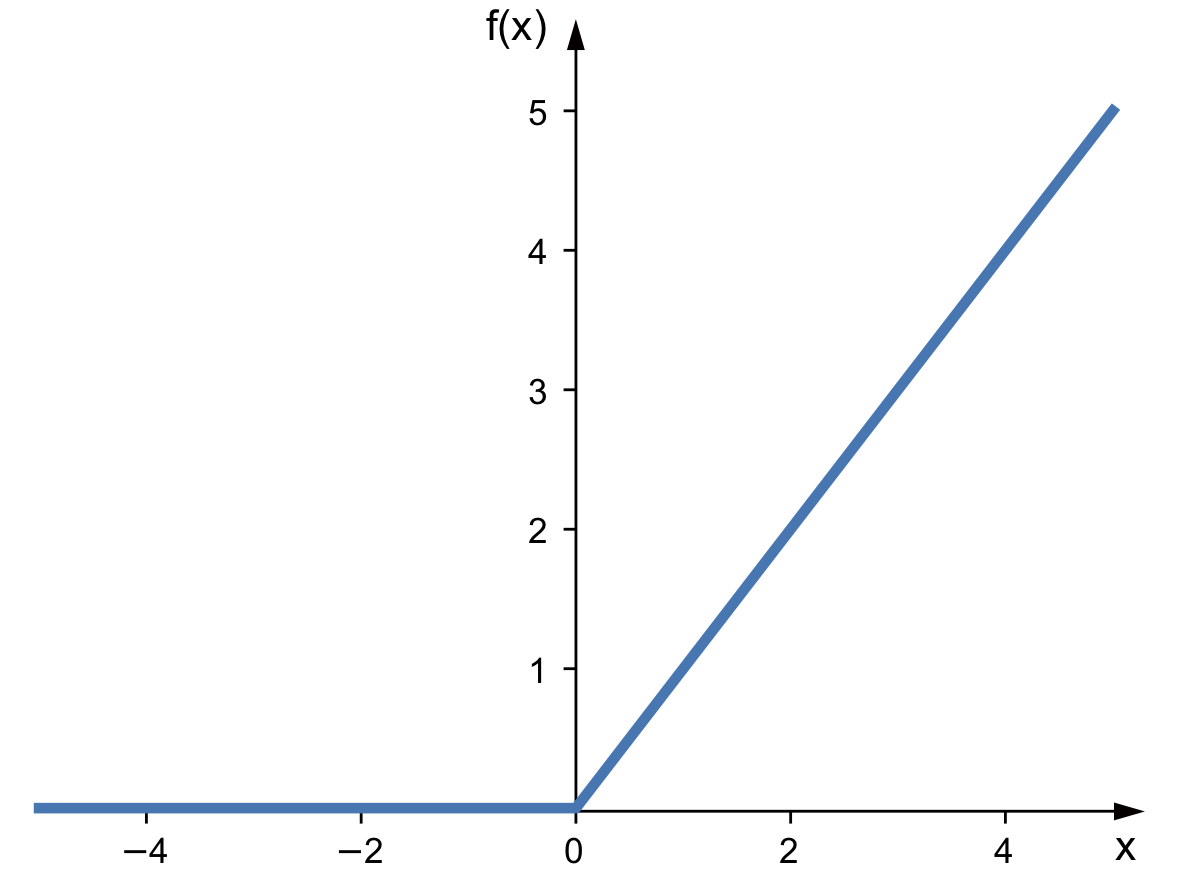
\includegraphics[width=\textwidth]{relu}
            \caption{Common activation function: ReLU, short for Rectified Linear Unit.}
        \end{subfigure}
    \end{figure}
\end{frame}


\section{Related}
\begin{frame}[c]{Based on PointNet}
    \Large
    A number of works build on PointNet \cite{qi2017pointnet}:
    \begin{itemize}
        \item Implementations and tools for visualization: \cite{charlesq342022Jun, aldipiroli2022Jun, yunxiaoshi2022Jun, Pytorch_Pointnet_Pointnet2}
        \item Further attempts at explaining what PointNet learned: \cite{zhang2019explaining, huang2019claim}
        \item Application of PointNet to different domains and problems: \cite{thiery2022medical, gutierrez2018deep, triess2021survey, liang2019multi, zhang2018collaborative, mrowca2018flexible}
    \end{itemize}
\end{frame}



\section{Complexity}
\begin{frame}[c]{Speed and Model Size}
    \large
    \begin{table}
    \centering
    % 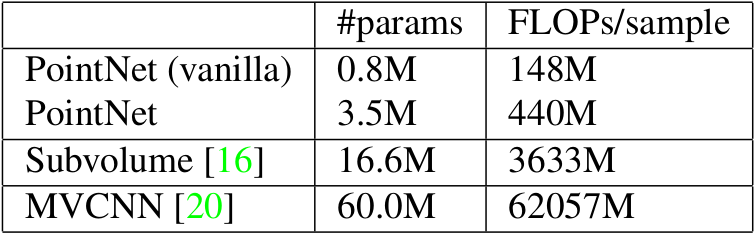
\includegraphics[width=0.4\textwidth]{complexity}
    \begin{tabular}{l|l|l}
        & \#params & FLOPs/sample \\ \hline
        PointNet (vanilla) & 0.8M & 148M \\
        PointNet & 3.5M & 440M \\ \hline
        Subvolume \cite{qi2016volumetric} & 16.6M & 3633M \\ \hline
        MVCNN \cite{su2015multi} & 60.0M & 62057M \\
    \end{tabular}
    \caption{
        \textbf{Time and space complexity of different deep learning
        architectures for 3D data classification.}
        PointNet (vanilla) is the classification PointNet without input and
        feature T-Net transformation networks. FLOP is floating-point
        operations. The ``M'' stands for a million units.
        Both Subvolume and MVCNN used input data pooling from multiple
        rotations or views, without which they have much inferior performance.
        % "\textbf{Time and space complexity of deep architectures for 3D data
        % classification.} PointNet (vanilla) is the classification PointNet
        % without input and feature transformations. FLOP stands for
        % floating-point operation. The “M” stands for million. Subvolume and
        % MVCNN used pooling on input data from multiple rotations or views,
        % without which they have much inferior performance."
        % Table and caption taken from \cite{qi2017pointnet}.
        % \todo{rewrite in own words}
        Table from \cite{qi2017pointnet}.
    } \label{table:complexity}
\end{table}

\end{frame}

\section{Permutation Invariance}
\begin{frame}[c]{Permutation Invariance: Sorting}
    \Large
    Unfortunately, there is no canonical order in high dim space.
    \begin{figure}
        \begin{tabular}{l|c}
            & Accuracy \\ \hline
            Unordered Input & 12\% \\
            Lexsorted Input & 40\% \\
            LSTM & 75\% \\
            PointNet (vanilla) & \textbf{87\%} \\
        \end{tabular}
        \caption{Validation on the ModelNet40 dataset. Table from CVPR presentation to \cite{qi2017pointnet}.}
    \end{figure}
\end{frame}

% \begin{frame}[c]{Experimentation: How about Sorting?}
%     order matters \cite{vinyals2015order}
%     \todo{would be additional slide, ignore for now}
%
%     \todo{include table of results with different 'sorting'/symmetric functions}
% \end{frame}

% \begin{frame}[c]{Experimentation: How about RNNs?}
%     \todo{would be additional slide, ignore for now}
%
%     \todo{include comparison table with LSTM}
%     \todo{Transformer: search if someone tried that?}
% \end{frame}


% \begin{frame}[c]{Semantic Segmentation in Scenes}
%     \begin{tabular}
%     mean IoU overall accuracy
% Ours baseline
% 20.12
% 53.19
% Ours PointNet
% 47.71
% 78.62
% Table 3. Results on semantic segmentation in scenes. Metric is
% average IoU over 13 classes (structural and furniture elements plus
% clutter) and classification accuracy calculated on points.
% \end{frame}
